\newpage

\section{Midsegments}
\begin{definition}
In a triangle, a \emph{midsegment} is a line joining the midpoints of two sides.  
\end{definition}

\begin{theorem}
Midsegment Theorem:  A midsegment in a triangle is parallel to and half the length of the corresponding side.
\end{theorem}

In this activity, we prove the midsegment theorem.  First, we need some results about parallelograms. 

\begin{prob}
Prove the following theorem:  If the diagonals of a quadrilateral bisect each other, then the quadrilateral is a parallelogram. 
\end{prob}

\begin{prob}
Prove the following theorem:  If one pair of sides of a quadrilateral are congruent and parallel, then the quadrilateral is a parallelogram. 
\end{prob}

\begin{prob}
Prove the midsegment theorem.  (Hint:  Extend the midsegment $\overline{DE}$ to a point $X$ such that $EX=DE$, and then find quadrilaterals that must be parallelograms by the previous results.)  
$$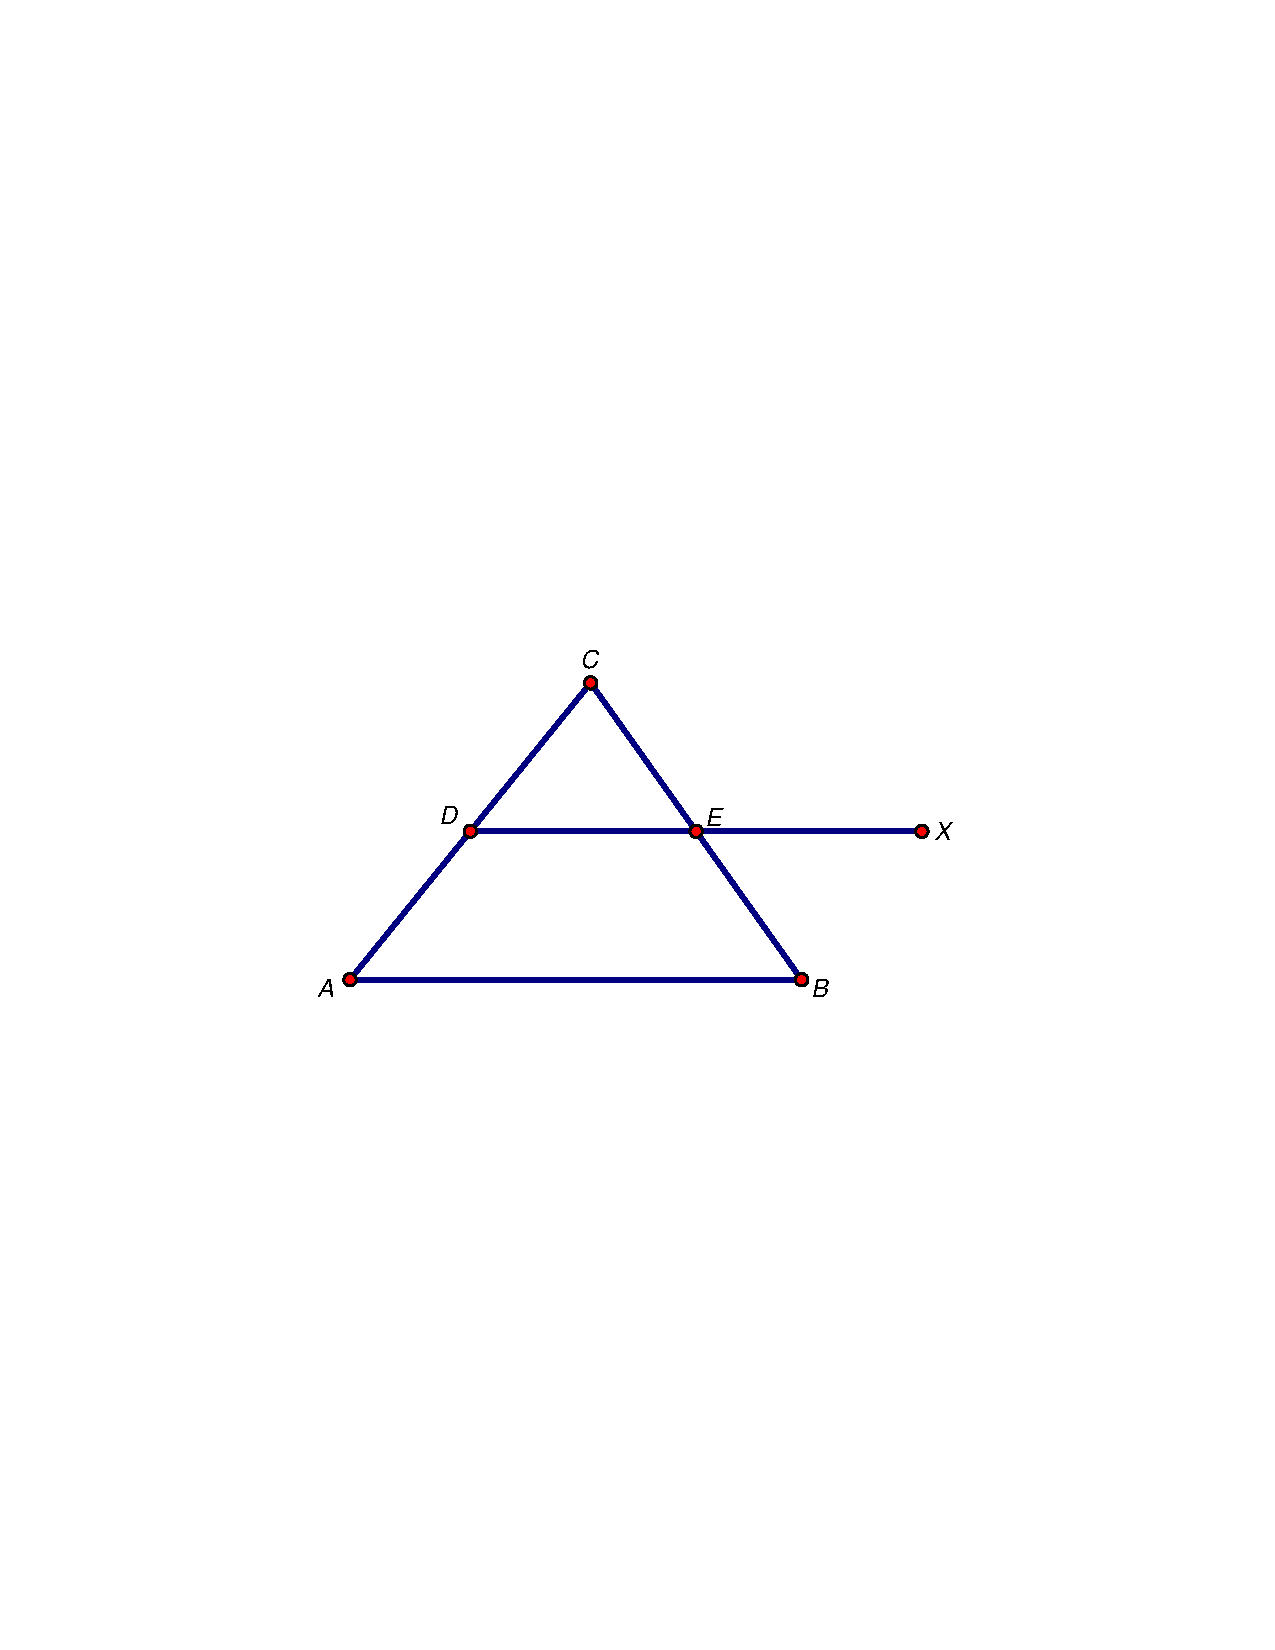
\includegraphics[scale=0.7]{../graphics/midsegment}$$
\end{prob}




